\documentclass[class=book, crop=false, oneside, 12pt]{standalone}
\usepackage{standalone}
\usepackage{amsmath}
\usepackage{../../style}
\graphicspath{{./assets/images/}}

% arara: pdflatex: { synctex: yes, shell: yes }
% arara: latexmk: { clean: partial }
\begin{document}

\chapter{Primo principio della termodinamica}

\section{Sistemi e stati termodinamici}

\subsection{Introduzione}

Un sistema termodinamico è spesso assimilabile, da un punto di vista meccanico, ad un sistema continuo, considerato che microscopicamente è costituito da un numero di elementi dell'ordine del \emph{numero di Avogadro}
\begin{equation*}
    N_A = 6.022 \cdot 10^{23}
\end{equation*}
Cercheremo invece di descrivere le trasformazioni che il sistema può subire e gli scambi energetici che ne risultano con l'ambiente circostante, individuando le grandezze più appropriate a tale descrizione.

\subsection{Sistema termodinamico}

Chiamiamo sistema termodinamico una porzione del mondo che può essere costituita da una o più parti, per esempio un volume di gas, un liquido in equilibrio con il suo vapore, un insieme di blocchi di solidi diversi; tale sistema è oggetto delle nostre osservazioni per quanto riguarda le proprietà fisiche macroscopiche che lo caratterizzano e le loro eventuali variazioni. 

\subsection{Ambiente e Universo}

Per ambiente circostante, o semplicemente ambiente, intendiamo quell'insieme che può essere costituito da una sola parte (per esempio l'aria o un altro fluido in cui è immerso il sistema) o da più parti (per esempio diversi corpi solidi a contatto con il sistema), con cui il sistema può interagire: l'ambiente pertanto contribuisce in generale a determinare le caratteristiche fisiche macroscopiche del sistema e la loro evoluzione.\newline
L'insieme sistema più ambiente si chiama \emph{universo termodinamico}, in senso locale.

\subsection{Sistema aperto}

Se tra il sistema e l'ambiente avvengono scambi di energia e di materia il sistema è detto aperto. 
Ad esempio, se il sistema è costituito da un liquido in ebollizione e l'ambiente dal recipiente che contiene il liquido, dall'atmosfera esterna compreso il vapore e dalla sorgente di calore, nel processo di ebollizione si ha trasformazione di liquido in vapore e quindi passaggio di materia dal sistema all'ambiente; 
inoltre vi è certamente passaggio di energia dall'ambiente al sistema tramite la sorgente di calore.

\subsection{Sistema chiuso}

Il sistema si dice chiuso se sono esclusi scambi di materia, ma si hanno solamente scambi di energia. 
Ritornando all'esempio precedente, il liquido è contenuto in un recipiente chiuso, a contatto con la sorgente di calore; il vapore prodotto rimane all'interno del sistema. 

\subsection{Sistema isolato}

Infine il sistema è detto isolato se non avvengono scambi di energia e di materia con un altro sistema esterno, cioè con l'ambiente. 
L'universo termodinamico formato da un sistema e dal suo ambiente è da considerarsi come un sistema isolato. 

\subsection{Variabili termodinamiche}

Un sistema termodinamico viene descritto tramite un numero ridotto di grandezze fisiche direttamente misurabili, dette coordinate o variabili termodinamiche, come volume, pressione, temperatura, massa, concentrazione, densità, ecc. 

Alcune variabili termodinamiche, chiamate variabili estensive, sono additive, come massa e volume; altre invece chiamate variabili intensive, dipendono in generale dalla posizione del punto nel sistema, e non sono additive.

Il numero minimo di coordinate termodinamiche necessario per descrivere completamente un sistema termodinamico non è fissato a priori, ma dipende dalle caratteristiche chimico-fisiche dei vari sistemi che vengono studiati. 
Le proprietà di un sistema vengono sempre espresse in funzione dei valori delle sue coordinate termodinamiche. 

Osserviamo che la definizione di stato termodinamico è concettualmente diversa da quella di stato meccanico, per il quale in linea di principio si presuppone la conoscenza di posizione e velocità di ciascuno degli \(n\) punti che costituiscono il sistema. 
In questi termini un sistema termodinamico non è definibile, visto il grande valore di \(n\). 
In effetti, se è noto lo stato termodinamico, non è noto in generale quello meccanico, anzi a un dato stato termodinamico possono corrispondere moltissimi stati meccanici diversi. 

\section{Equilibrio termodinamico, principio dell'equilibrio termico}

Lo stato termodinamico di un sistema è detto di equilibrio quando le variabili termodinamiche che lo descrivono sono costanti nel tempo. 
In un sistema termodinamico all'equilibrio le variabili termodinamiche sono dette variabili di stato.

\subsection{Equilibrio termodinamico}

L'equilibrio termodinamico è il risultato di tre diversi tipi di equilibrio, che devono essere realizzati contemporaneamente:

\begin{itemize}
    \item \emph{equilibrio meccanico}, inteso come equilibrio di forze e momenti, secondo quanto studiato in meccanica; 
    \item \emph{equilibrio chimico}: non avvengono reazioni chimiche o trasferimenti di un componente del sistema entro il sistema stesso; 
    \item \emph{equilibrio termico}: la temperatura è la stessa ovunque.
\end{itemize}

Se uno stato è di equilibrio, le condizioni di equilibrio devono essere soddisfatte all'interno del sistema o di ciascuna delle sue parti, nell'interazione tra le parti del sistema e in quella tra sistema e ambiente. 
Quando c'è equilibrio con l'ambiente, vuol dire che esiste equilibrio tra le forze macroscopiche, qualunque sia la loro natura, agenti dall'esterno sul sistema e quelle sviluppate dal sistema; 
inoltre la temperatura del sistema, se questo non è isolato termicamente, è eguale alla temperatura dell'ambiente. 

In uno stato di equilibrio esiste, in generale, una precisa relazione tra le coordinate termodinamiche che si esprime sotto forma di equazione di stato.

\subsection{Trasformazione termodinamica}

Dati due diversi stati di equilibrio termodinamico di un certo sistema, l'eventuale evoluzione del sistema dal primo al secondo stato, spontanea o per effetto dell'interazione con l'ambiente, si chiama trasformazione termodinamica del sistema. 
Considereremo sempre come stati iniziali e finali di una certa trasformazione stati di equilibrio. 

Invece gli stati intermedi attraverso cui passa il sistema durante l'evoluzione possono essere di equilibrio o di non equilibrio; in questo secondo caso non è detto che si possano determinare tutte le coordinate termodinamiche del sistema. 
Ai fini del calcolo si considerano anche trasformazioni infinitesime, tra stati molto prossimi, le cui coordinate differiscono di quantità infinitesime.

\subsection{Equilibrio termico}

Si considerino due sistemi \(A\) e \(B\), ciascuno in equilibrio termodinamico, con il sistema \(A\) alla temperatura \(T_A\) e quello \(B\) alla temperatura \(T_B\).
I sistemi si dicono in equilibrio termico tra loro quando hanno la stessa temperatura, \(T_A = T_B\): la temperatura è pertanto l'indice del'equilibrio termico tra due sistemi. 

È verificato sperimentalmente il seguente principio dell'equilibrio termico: due sistemi che siano ciascuno in equilibrio termico con un terzo sistema sono in equilibrio termico tra loro. 
Se il sistema \(A\) è in equilibrio termico con il sistema \(C\) (\(T_A = T_C\)) e se anche il sistema \(B\) è in equilibrio termico con \(C\) (\(T_B = T_C\)), allora \(A\) è in equilibrio termico con \(B\) ( \(T_A = T_B\)).

Un metodo possibile per portare due sistemi all'equilibrio termico è quello di tenerli a contatto, tramite una parete. 
Se viene raggiunto l'equilibrio termico si parla di \emph{parete diatermica}, mentre se non si raggiunge mai l'equilibrio termico, e pertanto le due temperature sono indipendenti, la parete è detta \emph{adiabatica}. 
Nella realtà la situazione adiabatica è un caso limite, che può essere realizzato per tempi brevi, ma non in assoluto.

\subsection{Contatto termico}

Due sistemi separati da una parete diatermica si dicono anche in contatto termico tra loro e inevitabilmente raggiungono l'equilibrio termico. 
Il contatto termico si può realizzare anche direttamente, senza alcuna parete, come avviene per due corpi solidi a contatto, per un corpo solido immerso in un fluido o per due fluidi non miscibili a contatto; la parete diatermica si rende necessaria quando bisogna contenere il sistema, come avviene nel caso di un gas. 

\subsection{Sistema adiabatico}

Un sistema è detto adiabatico se è circondato da pareti adiabatiche e quindi non può essere messo in contatto termico con un altro sistema o  con l'ambiente. 
Una parete è sempre necessaria per impedire o ritardare l'equilibrio termico. 

Notiamo infine che l'esistenza di equilibrio termico tra due sistemi non presuppone affatto che essi siano anche in altri tipi di equilibrio, ne viceversa.

\section{Definizione temperatura, termometri}

Per fare una definizione operativa di temperatura devono essere realizzate due condizioni. 
Deve esistere una grandezza \(X\) che caratterizza un fenomeno fisico e che varia con la temperatura. 
\(X\) si chiama \emph{caratteristica termometrica} e la temperatura è una funzione di \(X\), \(\theta (X)\), detta \emph{funzione termometrica}. 
Il dispositivo in cui avviene il fenomeno e che fornisce il valore della caratteristica termometrica è indicato come \emph{termometro}.

\subsection{Punto fisso}

In secondo luogo deve esistere un sistema, in uno stato di equilibrio, definibile con precisione e riproducibile con facilità, cui viene attribuito un valore arbitrario di temperatura, detto \emph{punto fisso}.

Il punto fisso campione è il \emph{punto triplo} dell'acqua, ovvero quel particolare stato in cui ghiaccio, acqua e vapor d'acqua saturo sono in equilibrio. 
Al punto triplo dell'acqua è stata assegnata arbitrariamente la temperatura di \(273.16 K\), dove il simbolo \(K\) indica l'unità di misura prescelta, il kelvin.

\subsection{Misura della temperatura}

Per arrivare a esprimere numericamente la temperatura stabiliamo in via preliminare che la forma della funzione \(\theta(X)\) sia \(\theta(X) = aX\), con \(a\) costante.
È la scelta più semplice, giustificata però dal fatto che è valida per il termometro assoluto.

Il sistema, di cui vogliamo misurare la temperatura, viene messo a contatto termico con un termometro che, all'equilibrio termico, fornisce il valore \(X\).

Tale termometro al punto triplo dell'acqua dà il valore \(X_{pt}\) e per definizione abbiamo
\begin{equation*}
    \theta (X_{pt}) = a X_{pt} = 273.16
\end{equation*}
da cui \(a = 273.16/X_{pt}\), valore valido per quel termometro. Ne segue che la temperatura \(T\) del sistema, espressa dal valore della funzione \(\theta (X) = a X\), si scrive
\begin{equation}
    T = 273.16 \frac{X}{X_{pt}} K    
\end{equation}

L'ultima formula è la formula fondamentale per ogni termometro e fornisce la temperatura empirica di quel termometro.

Si usa il termine temperatura empirica in quanto, sperimentalmente, si constata che termometri di tipo diverso, o anche due diversi termometri dello stesso tipo, danno sempre letture diverse quando sono in equilibrio termico con lo stesso stato di un certo sistema, pur dando per costruzione tutti la stessa temperatura al punto triplo dell'acqua.
Se si vuole verificare se due sistemi sono alla stessa temperatura si deve metterli uno alla volta in contatto termico con lo stesso termometro. 

\subsection{Scale termometriche}

La scala che viene più comunemente usata nelle normali misure di temperatura è quella Celsius, in cui la temperatura del punto triplo dell'acqua vale \(0.01\) gradi Celsius (simbolo \(^{\circ} C\)).
Pertanto lo zero della scala Celsius è a \(273.15 K\) e corrisponde alla temperatura di fusione del ghiaccio a pressione atmosferica. 

Il valore di una differenza di temperatura è assunto lo stesso in gradi Celsius o in kelvin e pertanto la formula di conversione dal valore in kelvin \(T (K)\) al valore in gradi Celsius \(t ( ^{\circ} C)\) è semplicemente
\begin{equation*}
    t (^{\circ} C) = T (K) - 273.15
\end{equation*}

Nei paesi anglosassoni vengono utilizzate altre due scale di temperatura, la scala Rankine \(t ( ^{\circ} R)\) e la scala Fahrenheit \( t ( ^{\circ} F)\), che sono così definite rispetto alla temperatura espressa in kelvin:
\begin{equation*}
    t ( ^{\circ} R) = \frac{9}{5} T (K)
\end{equation*}
\begin{equation*}
    t (^{\circ} F) = \frac{9}{5} T (K) - 459.67
\end{equation*}

Il legame tra scala Fahrenheit e scala Celsius è pertanto:
\begin{equation*}
    t (^{\circ} F) = \frac{9}{5} t (^{\circ} C) + 32 \ , \ t(^{\circ} C) = \frac{5}{9} \left[t (^{\circ} F ) - 32\right]
\end{equation*}

Nella scala Fahrenheit il punto di fusione del ghiaccio (\(0 ^{\circ} C \)) corrisponde a \(32 ^{\circ} F\) e il punto di ebollizione dell'acqua (\(100 ^{\circ} C\)) a \(212 ^{\circ} F\); la temperatura ambiente di \(20 ^{\circ} C\) vale \(68 ^{\circ} F\). 

\section{Sistemi adiabatici, esperimenti di Joule, Calore}

\subsection{Esperimenti di Joule}

Joule condusse una serie di esperimenti fondamentali sugli effetti termici del lavoro meccanico. 
Schematicamente, le varie esperienze eseguite da Joule su un sistema termodinamico costituito da una certa quantità d'acqua avevano lo scopo di realizzare un aumento della temperatura del sistema con procedimenti diversi. 

\begin{itemize}
    \item Viene messo in rotazione un mulinello nell'acqua spendendo il lavoro \(W_1\), fornito dalla variazione di energia potenziale di due masse che scendono sotto l'azione della forza di gravità. 
    Con varie palette fisse immerse nell'acqua si impedisce che essa entri in rotazione. 
    L'acqua, agitata dal mulinello, viene riscaldata per effetto dell'attrito. 
    \item Viene immerso nell'acqua un conduttore di resistenza \(R\), percorso da corrente. 
    \(W_2\) è il lavoro speso per fare circolare la corrente.
    \item Viene compressa una certa quantità di gas, contenuta in un recipiente con pareti diatermiche, immerso nell'acqua. 
    Il processo di compressione del gas richiede un lavoro.
    \item Vengono strofinati tra loro due blocchi di metallo immersi nell'acqua.  
    Il lavoro speso contro le forze di attrito è \(W_4\).
\end{itemize}
Nelle varie esperienze l'insieme costituito dall'acqua e dal dispositivo meccanico o elettrico è racchiuso entro pareti adiabatiche. 

Il risultato fondamentale osservato da Joule è che il lavoro speso a parità di massa d'acqua, \(W_1\) o \(W_2\) o \(W_3\) o \(W_4\), è sempre proporzionale alla variazione di temperatura dell'acqua con la stessa costante di proporzionalità.\newline
Il sistema termodinamico \emph{massa d'acqua} passa da uno stato iniziale di equilibrio, caratterizzato dal valore \(T_{in}\) della temperatura, ad uno stato finale di equilibrio con temperatura \(T_{fin}\) tramite quattro diversi processi, ma il lavoro meccanico è sempre lo stesso.

Sulla base delle considerazioni per l'energia potenziale nel caso di forze conservative, scriviamo la seguente relazione:
\begin{equation}
    W_{ad} = - \Delta U = U_{in} - U_{fin} \udm{J}
\end{equation}
dove \(U\) è una funzione che dipende solo dallo stato del sistema cioè dalle sue coordinate termodinamiche.

Se il sistema fornisce lavoro all'esterno, \(W\) è assunto positivo e pertanto l'energia \(U\) diminuisce; se invece si compie lavoro dall'esterno sul sistema \(W\) è assunto negativo e l'energia \(U\) aumenta.

Se possiamo ottenere lo stesso cambiamento di stato termodinamico dell'acqua, segnalato dalla stessa variazione di temperatura, tramite scambio di calore o di lavoro meccanico, possiamo postulare l'equivalenza degli effetti delle due procedure e scrivere anche nel caso di scambio di calore con lavoro nullo, una relazione analoga a:
\begin{equation}
    Q = \Delta U
\end{equation}
assumendo positivo il calore ceduto al sistema dall'esterno. 

\subsection{Equivalenza calore e lavoro}

Pertanto 
\begin{equation}
    Q = -W
\end{equation}
dove rappresenta il calore scambiato, senza lavoro esterno per far variare di \(\Delta T\) la tempratura della massa d'acqua e \(W\) il lavoro che deve essere speso, in condizioni adiabatiche, per ottenere la stessa variazione di temperatura. 

L'ultima equazione è detta \emph{equivalenza tra calore e lavoro}; essa indica anche come si possa eseguire una misura del calore scambiato. 
Il calore viene in questo modo espresso in joule \(\udm{J}\).

\section{Primo principio della termodinamica, energia interna}

\subsection{Primo principio della termodinamica}

Si abbia un sistema che oltre allo scambio di lavoro meccanico con l'ambiente possa avere anche scambio di calore, cioè trasmissione di energia non accompagnata da fenomeni meccanici macroscopici.
Il sistema compie una trasformazione dallo stato \(A\) allo stato \(B\), scambiando calore e lavoro con l'ambiente, \(Q\) e \(W\) dipendono dalla trasformazione che congiunge i due stati termodinamici, mentre invece la differenza \(Q-W\) risulta indipendente dalla trasformazione. 

Si può scrivere posto \(\Delta U = U_B - U_A\):
\begin{equation} \label{primo_principio_termodinamica}
    Q - W = \Delta U \ , \ Q = \Delta U + W
\end{equation}
che esprime il \emph{primo principio della termodinamica}

\subsection{Implicazioni del primo principio}

Le implicazioni del primo principio della termodinamica possono essere sviluppate su più punti:
\begin{enumerate}
    \item Esiste una funzione delle coordinate termodinamiche del sistema o, come si dice, una funzione di stato, chiamata energia interna, le cui variazioni danno gli scambi energetici del sistema con l'ambiente che lo circonda durante una trasformazione. 
    Dati due stati \(A\) e \(B\) è fissata \(\Delta U\): in una particolare trasformazione dallo stato \(A\) a quello \(B\) può essere preponderante lo scambio di calore, mentre in un'altra trasformazione, sempre tra tali stati, quello di lavoro, però in ambedue le diverse trasformazioni lo scambio totale \(Q - W\) è lo stesso. 
    \item Quando, durante una trasformazione, si fornisce energia a un sistema, sia tramite un lavoro meccanico che con uno scambio di calore, questa resta immagazzinata sotto forma di energia interna e può essere successivamente riutilizzata.
    Possiamo dire che la (\ref{primo_principio_termodinamica}) costituisce l'espressione del bilancio energetico di una trasformazione termodinamica; si tratta di un bilancio più completo di quello che è possibile fare in meccanica, in quanto si tiene conto anche degli scambi di calore.
    \item Il termine energia interna indica che non si tratta dell'energia cinetica o potenziale bensì di energia legata a proprietà interne del sistema, come moto molecolare o forze intermolecolari, che non dipendono dallo stato complessivo di moto, ma piuttosto dalla temperatura del sistema, dalla pressione a cui è sottoposto o dal volume che occupa. 
    È importante osservare che l'espressione esplicita dell'energia interna in funzione delle coordinate termodinamiche che individuano lo stato di un sistema dipende dal sistema stesso.
    \item Il primo principio mette in evidenza l'esistenza di un meccanismo di scambio di energia, che non è esprimibile come lavoro meccanico macroscopico: a questo diamo il nome di calore. 
    Esso è ancora riconducibile a fenomeni meccanici, ma a livello microscopico.
    Bisogna prestare attenzione al fatto che il calore e il lavoro sono forme di scambio di energia e quindi si deve sempre parlare di calore o lavoro scambiati tra sistemi e mai di calore o lavoro posseduti da un sistema. 
    Ciò che un sistema possiede è una certa quantità di energia che può variare in una trasformazione, appunto a seguito di scambi di calore e lavoro.
    \item Se un sistema termodinamico esegue una qualsiasi trasformazione che lo riporti allo stato iniziale, ovvero una trasformazione ciclica o chiusa, si ha per definizione
    \begin{equation}
        \Delta U = 0 \implies Q = W
    \end{equation}
    Il calore scambiato è eguale al lavoro scambiato. 
    Se nella trasformazione ciclica il sistema complessivamente assorbe calore, \(Q > 0\), esso fornisce lavoro, \(W > 0\), costituisce una macchina termica. 
    \item Per eseguire calcoli specifici è assai utile considerare trasformazioni termodinamiche nelle quali le variabili di stato cambiano di quantità infinitesime.
    Il primo principio ha la forma:
    \begin{equation*}
        \delta Q = d U + \delta W
    \end{equation*}
    Integrando per una trasformazione finita si ha:
    \begin{equation*}
        \Delta U = \int_A^B d U = U_B - U_A
    \end{equation*}
    indipendente dalla trasformazione, mentre invece, come sappiamo:
    \begin{equation*}
        Q_{AB} = \int_A^B \delta Q
    \end{equation*}
    la variazione infinitesima di energia interna è un differenziale esatto, mentre \(\delta Q \) e \(\delta W\), cioè le quantità infinitesime di calore e lavoro scambiati, non sono differenziali esatti perché sono grandezze che dipendono dal percorso (essendo funzioni di percorso).
    \item L'unità di misura di energia interna, calore e lavoro è la stessa, il Joule.
\end{enumerate}

\subsection{Convenzione segni lavoro e calore}

Naturalmente quello che importa in una trasformazione è capire qual è il flusso energetico, cioè se il calore è assorbito o ceduto dal sistema, se il lavoro è prodotto o subito, in modo da poter correttamente pervenire al bilancio energetico. 
I segni sono solo convenzionali, però scelta una certa convenzione questa va mantenuta in tutti i ragionamenti.

Attenzione che qui si considerano \emph{flussi di energia dal sistema}. 
Se il sistema assorbe calore, e diciamo che \(Q\) è positivo, questo calore è ceduto al sistema dall'ambiente e pertanto per l'ambiente è negativo e come tale dobbiamo trattarlo se ragioniamo sull'ambiente: se \(Q\) è il calore scambiato dal sistema, \(-Q\) è  quello scambiato dall'ambiente. 
Un discorso analogo va fatto per il lavoro.

\begin{figure}[h]
    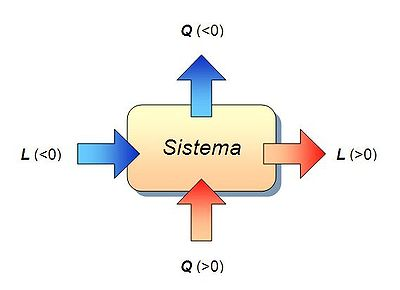
\includegraphics[scale=0.8]{termodinamica1}
    \centering
\end{figure}

Ricapitolando:

\begin{table}[h]
    \centering
    \begin{tabular}{|l|l|}
    \hline
    \textbf{Flusso di energia}                       & \textbf{Segno} \\ \hline
    Calore che entra in un sistema dall'esterno      & Positivo       \\ \hline
    Lavoro che è compiuto da un sistema sull'esterno & Positivo       \\ \hline
    Calore che esce da un sistema verso l'esterno    & Negativo       \\ \hline
    Lavoro che è compiuto dall'esterno sul sistema   & Negativo       \\ \hline
    \end{tabular}
    \caption{Convenzione sui segni di Q e W}
    \label{tab:convenzione_segni}
\end{table}

\section{Trasformazioni termodinamiche, lavoro e calore}

Abbiamo definito una trasformazione come un passaggio del sistema attraverso diversi stati, ovvero come un processo in cui cambiano le coordinate termodinamiche, qualcuna o tutte, del sistema.
Il primo principio della dinamica fissa il bilancio energetico di tale processo e infatti, oltre a definire una trasformazione, siamo interessati a calcolare quanto valgono \(\Delta U, W\) e \(Q\). 

La quantità \(\Delta U\) può essere calcolata direttamente se è nota l'espressione esplicita di \(U\), altrimenti l'unico modo possibile è servirsi di del primo principio, conoscendo quindi il calore e il lavoro scambiati. 
Però \(\Delta U\) non deve necessariamente essere calcolata lungo la data trasformazione, bensì lungo una qualsiasi altra che abbia gli stessi stati iniziale e finale e per la quale risulti più facile determinare \(Q\) e \(W\): 

L'espressione del primo principio viene dunque usata in definitiva come equazione ad una incognita e deve essere collegata a relazioni che permettono il calcolo delle altre due quantità.

\subsection{Trasformazioni adiabatiche}

Si chiama trasformazione adiabatica una qualsiasi trasformazione in cui \(Q = 0\), cioè dove il sistema non scambia calore con l'esterno, ossia è isolato termicamente dall'esterno.
Sistema adiabatico è un sistema che compie solo trasformazioni adiabatiche e per il quale quindi il primo principio si scrive \(W = - \Delta U\).
Gli scambi energetici con l'ambiente possono avvenire solo sotto forma di lavoro meccanico. 

Sperimentalmente questa situazione si realizza chiudendo il sistema in un contenitore con pareti adiabatiche. 
Infatti, richiamando quello visto precedentemente:

\begin{enumerate}
    \item una trasformazione che porta all'equilibrio termico avviene con scambio di calore; 
    \item una parete diatermica permette il passaggio di calore da un sistema all'altro: è quindi una parete conduttrice di calore;
    \item una parete adiabatica non permette il passaggio calore: è quindi isolante rispetto allo scambio di calore;
\end{enumerate}

Nella pratica l'adiabaticità perfetta non esiste; tutte le sostanze con cui si realizzano pareti adiabatiche permettono un certo scambio di calore. 
Si ammette che possa essere adiabatica una trasformazione che avviene rapidamente, così che non ci sia tempo per scambi di calore apprezzabili. 

\subsection{Trasformazioni reversibili e irreversibili}

Per effettuare una trasformazione che passi attraverso stati di equilibrio bisogna procedere con variazioni molto piccole delle coordinate termodinamiche, in modo che queste siano in pratica definite in ogni istante.
Ciò si può realizzare distaccandosi molto poco da uno stato di equilibrio, per permettere che la trasformazione avvenga, e attendendo il ristabilirsi dell'equilibrio nelle nuove condizioni prima di procedere a un'ulteriore variazione infinitesima di stato. 
Ne consegue che la trasformazione deve svolgersi lentamente.

La lentezza della trasformazione come condizione necessaria non è certamente sufficiente.
Oltre all'esame delle condizioni di equilibrio o non equilibrio si deve verificare durante la trasformazione l'eventuale presenza di \emph{forze dissipative}, come attriti che si oppongono allo spostamento di parti meccaniche durante lo scambio di lavoro, attriti viscosi, ecc.

In alternativa possiamo classificare le trasformazioni secondo il seguente schema:

\begin{enumerate}
    \item una trasformazione è detta \emph{reversibile} se essa avviene attraverso stati di equilibrio e in assenza di qualsiasi forza dissipativa; 
    \item una trasformazione è detta \emph{irreversibile} qualora non si svolga secondo le modalità precedenti.
    Ossia passi attraverso stati di non equilibrio o avvenga in presenza di forze dissipative oppure si verifichino, durante il suo svolgimento, entrambe queste situazioni. 
\end{enumerate}
Le trasformazioni reversibili sono casi limite, utilissime concettualmente per i calcoli, ma difficilmente realizzabili.

Una trasformazione reversibile può essere arrestata in qualunque stato intermedio e, variando di poco le condizioni esterne, si può invertire il verso della trasformazione, ripercorrendo gli stessi stati già attraversati.  
In tal caso cambia il segno degli scambi di energia e della variazione di energia interna.

\section{Calorimetria}
Il primo principio della termodinamica introduce e definisce la grandezza fisica calore, mettendo in evidenza che, in generale, lo scambio di calore comporta per un sistema una variazione di energia interna e uno scambio di lavoro secondo, offrendo anche un modo esplicito per effettuare il calcolo.

Esistono però processi particolari, e molto comuni, in cui è possibile ricavare un'espressione analitica del calore scambiato direttamente in funzione della variazione delle coordinate termodinamiche nella trasformazione.

Un esempio possono essere due corpi a diversa temperatura che vengono messi in contatto termico all'interno di un contenitore adiabatico. 
Nel processo viene raggiunto la temperatura di equilibrio \(T_e\).

Nel processo non viene scambiato lavoro né con l'ambiente né tra i due corpi, se ammettiamo che le variazioni di volume dei due corpi siano trascurabili; inoltre i due corpi non scambiano calore con l'ambiente. 
Pertanto \(Q\) e \(W\) sono nulli e l'energia interna totale del sistema, costituito dai due corpi, resta costante.

Le rispettive energie interne dei due corpi \(\Delta U_1\) e \(\Delta U_2\) però cambiano.
Dovendo essere \(\Delta U = \Delta U_1 + \Delta U_2 = 0\) abbiamo \(\Delta U_1 = - \Delta U_2\) le variazioni di energia interna dei due corpi sono eguali in modulo ed opposte.
Inoltre applicando il primo principio della termodinamica si ha che \(\Delta U_1 = Q_1\) e \(\Delta U_2 = Q_2\): il calore scambiato dal primo corpo è uguale ed opposto a quello scambiato dal secondo \(Q_1 = Q_2\).

D'altra parte gli esperimenti di Joule fanno ritenere che l'energia interna cresca con la temperatura, per cui \(\Delta U_1 < 0 \) e \(\Delta U_2 > 0 \):
in conclusione possiamo affermare che il calore ceduto dal primo corpo, il corpo più caldo, è eguale in modulo a quello assorbito dal secondo corpo, più freddo. 

Per effettuare la misura del calore scambiato viene effettuata la seguente metodologia:
\begin{enumerate}
    \item si cede \(Q_1\) ad una massa d'acqua, ponendo il corpo a contatto termico con l'acqua per il tempo necessario alla variazione \(T_e - T_1\), di temperatura del corpo; 
    in corrispondenza anche l'acqua subisce una variazione di temperatura \(\Delta T\), con \(\Delta T\) non necessariamente eguale a \(T_e - T_1\) (in modulo);
    \item si misura, per esempio con uno dei dispositivi di Joule, il lavoro \(W_2\) necessario per produrre la stessa variazione \(\Delta T\) nella stessa massa d'acqua; 
    \item si pone \(| Q_1 | = W_2\)
\end{enumerate}

Nel realizzare queste misure si trova che esiste proporzionalità tra il calore \(Q\), la massa del corpo stesso e la variazione della sua temperatura:
\begin{equation} \label{prop_q_m_dT}
    Q = m c \left(T_{fin} - T_{in}\right)
\end{equation} 
dove \(c\) è una grandezza caratteristica della sostanza di cui è costituito il corpo, in generale funzione a sua volta della temperatura, chiamata \emph{calore specifico}.
Osserviamo che il calore è una grandezza estensiva, mentre il calore specifico è una grandezza intensiva.

Il calore specifico rappresenta il calore che occorre scambiare con l'unità di massa di una data sostanza, alla temperatura \(T\), per farne variare la temperatura di \(1 K\) (ovvero di \(1 ^{\circ} C\))

Il prodotto \(C = mc\), detto \emph{capacità termica del corpo}, rappresenta a sua volta il calore necessario per far variare di \(1 K\) la temperatura del corpo.

Posso riscrivere (\ref{prop_q_m_dT}) in termini infinitesimi:
\begin{equation}
    d Q = m c d T
\end{equation}
essendo \( d Q \) il calore infinitesimo scambiato dalla massa \(m\) alla temperatura \(T\) e \(d T\) la corrispondente variazione infinitesima di temperatura.

Da quest'ultima equazione segue per il calore specifico:
\begin{equation}
    c = \frac{1}{m} \frac{d Q}{d T}
\end{equation}

Ritornando ai due corpi in contatto termico, l'eguaglianza \(Q_1 = -Q_2\) diviene in base a 
\begin{equation*}
    m_1 c_1 (T_e - T_1) = - m_2 c_2 \left(T_e - T_2\right)
\end{equation*}
da cui, noti i calori specifici e misurate le masse e le temperature iniziali, si può calcolare la temperatura finale di equilibrio \(T_e\).

Il risultato trovato si può generalizzare: quando un corpo solido o liquido presenta una variazione di temperatura da \(T_1\) a \(T_2\) a seguito del contatto termico con un altro corpo, ammettiamo che abbia scambiato il calore
\begin{equation}
    Q = m c \left(T_2 - T_1\right)
\end{equation}
essendo \(m\) la sua massa e \(c\) il suo calore specifico. 
Il calore risulta assorbito se \(T_2 > T_1\), ceduto se \(T_2<T_1\). 
Qualora nell'intervallo di temperatura da \(T_1\) a \(T_2\) si possa assumere che il calore specifico sia praticamente costante bisogna invece scrivere
\begin{equation}
    Q = \int d Q = m \int_{T_1}^{T_2} c(T) d T
\end{equation} 

\section{Processi isotermi, cambi di fase}

\subsection{Processi isotermi}

Una trasformazione isoterma è una trasformazione termodinamica a temperatura costante, ossia una variazione dello stato di un sistema fisico durante la quale la temperatura del sistema non varia nel tempo.
Una classe importante di processi isotermi è costituita dai cambiamenti di fase, ovvero dai passaggi di una sostanza da una fase all'altra, per esempio dalla fase solida alla fase liquida o dalla fase liquida a quella di vapore.

\subsection{Cambi di fase}

\begin{itemize}
    \item solido \(\implies\) liquido : fusione
    \item liquido \(\implies\) solido : solidificazione
    \item liquido \(\implies\) vapore : evaporazione
    \item vapore \(\implies\) liquido : condensazione
    \item solido \(\iff\) vapore :  sublimazione
\end{itemize}

Alcuni cambiamenti di fase, come fusione e solidificazione, che avvengono a una determinata temperatura, costante durante il processo, costituiscono un punto di riferimento (punto fisso) per le scale termometriche, purché siano ben precisate le condizioni esterne, soprattutto la pressione.

L'evaporazione di un liquido ha luogo invece a qualsiasi temperatura; essa assume un carattere particolare solo quando la pressione massima del vapore eguaglia la pressione esterna: si ha in tal caso l'ebollizione che avviene a una ben determinata temperatura, dipendente dalla pressione esterna. 

Nella definizione della scala Celsius si era utilizzato il punto fisso fornito dal ghiaccio fondente a pressione atmosferica, posto eguale a \(0 ^{\circ} C\), e quello corrispondente all'ebollizione dell'acqua a pressione atmosferica, posto eguale a \(100 ^{\circ} C\)

I cambiamenti di fase sono accompagnati da scambi di calore e si osserva che per unità di massa, si tratta di quantità definite, dette calori latenti \(\lambda\). 
Pertanto il calore richiesto per il cambiamento di fase della massa \(m\) di una sostanza pura è dato da
\begin{equation}
    Q = m \lambda
\end{equation}

Il calore \(Q\) deve essere ceduto alla sostanza per fare avvenire, ad esempio, la fusione o sottratto alla sostanza per produrre la solidificazione.\newline
Nel caso dell'evaporazione il calore latente non ha un valore fisso, ma è una funzione decrescente della temperatura e si annulla alla temperatura critica.\newline
Una caratteristica molto importante dei cambiamenti di fase è di essere, in opportune condizioni, trasformazioni praticamente reversibili.

\section{Trasmissione del calore}

Il primo principio della termodinamica riguarda gli scambi energetici che av-vengono durante una trasformazione termodinamica. Lo scambio di lavoro concerne il lavoro meccanico macroscopico legato allo spostamento di qualche oggetto, ad esempio la parete mobile di un recipiente pieno di gas. 
Lo scambio di calore presuppone invece un meccanismo microscopico, cui accenneremo in seguito, e avviene quando due corpi sono a contatto direttamente o attraverso altri corpi.
Lo scambio e anche il trasporto di calore entro un sistema possono avvenire tramite tre meccanismi distinti, che nel loro complesso sono indicati come trasmissione calore: conduzione, convezione e irraggiamento termici.

I tre meccanismi operano sempre in presenza di una differenza di temperatura tra sistema e ambiente o all'interno dello stesso sistema. 

\subsection{Conduzione di calore}

Consideriamo un corpo esteso in cui la temperatura non sia uniforme e tracciamo le superfici isoterme cioè il luogo dei punti in cui la funzione \(T(x,y,z)\) assume un valore costante.

Se \(d S\) è una superficie isoterma, \(d T / d n\) il modulo del gradiente temperatura, ortogonale a \(d S\) e diretto nel verso delle temperatura, il calore che passa attraverso \(d S\) nel tempo \(d t\) è dato da
\begin{equation}
    d Q = - k \frac{d T }{d n} d S d t
\end{equation}
la grandezza \(k\), detta \emph{conducibilità} o \emph{conduttività termica}, è tipica del materiale ed è in generale funzione della temperatura.
Il segno negativo indica che il flusso di calore avviene nel senso in cui la temperatura diminuisce, cioè nel verso opposto al gradiente di temperatura, dalla regione a temperatura maggiore a quella a temperatura minore.

La conducibilità termica varia da sostanza a sostanza anche di diversi ordini di grandezza.
La conducibilità termica ha una diversa dipendenza dalla temperatura per le varie sostanze. 
Nei gas semplici \(k\) cresce debolmente con la temperatura, in proporzione alla radice quadrata della stessa. 
Anche nei liquidi e nei dielettrici non vi è una notevole variazione con la temperatura. 
Nei metalli puri la conducibilità presenta sempre un massimo a bassa temperatura, che è due o tre ordini di grandezza maggiore del valore a temperatura ambiente.

Attraverso una superficie finita \(S\) nel tempo \(t\) passa dall'ambiente posto a sinistra della parete a quello a destra il calore 
\begin{equation*}
    Q = k \frac{T_1 - T_2}{s} S t
\end{equation*}

\subsection{Convezione di calore}

La conduzione nei fluidi è difficile da osservare perché in essi si manifesta un altro fenomeno di trasmissione del calore, la convezione.

Se si riscalda una massa fluida, quella parte più vicina alla sorgente di calore assume una temperatura maggiore e diminuisce di densità, dilatandosi. 
Viene alterato l'equilibrio statico nel fluido, poiché gli elementi di fluido più caldi risentono, dalle parti di fluido circostante più fredde, una spinta di Archimede maggiore del loro peso. 
Si originano correnti ascensionali (dette di convezione), che permettono ad elementi con temperatura minore di avvicinarsi a loro volta alla sorgente di calore. 
La trasmissione di calore avviene con spostamenti di materia, tramite correnti convettive. 

La convezione è responsabile del movimento delle masse d'aria nell'atmosfera o delle correnti marine, con effetti sulle condizioni climatiche e metereologiche.

\subsection{Irraggiamento}

Un corpo a temperatura \(T\) emette energia sotto forma di onde elettromagnetiche, che si propagano nello spazio circostante, anche se vuoto. 
Il potere emissivo del corpo \(P\), che ha il significato di energia emessa per unità di tempo e per unità di superficie, è dato dalla legge di Stefan-Boltzmann: 
\begin{equation}
    P = \sigma e T^{4}
\end{equation}
dove \(\sigma\) è una costante universale, pari a  \(5.67 \cdot 10^{-8} \frac{J}{m^2 s K^4}\), ed \(e\) una grandezza, detta potere emissivo specifico, che può variare tra \(0\) e \(1\), dipendendo dalle proprietà della superficie. 
Se \(e = 1\), la superficie è detta superficie nera e presenta, a parità di temperatura, il massimo potere emissivo. 

Tramite questi fenomeni la temperatura di un corpo aumenta o diminuisce a seconda del bilancio tra energia irradiata ed assorbita; se il bilancio è in parità la temperatura resta costante, il corpo è in equilibrio con l'ambiente circostante. 
Naturalmente l'equilibrio può essere mantenuto anche fornendo o sottraendo energia con altri mezzi, per compensare l'irraggiamento. 
È attraverso il meccanismo dell'irraggiamento che il sole trasmette energia alla superficie terrestre, nella misura di \(1.53 \cdot 10^3 \frac{J}{m^2 s}\).

\subsection{Parete adiabatica, Vaso di Dewar}

Vediamo in base ai vari effetti studiati come è possibile realizzare una parete adiabatica. 
Se lo scopo è quello di limitare lo scambio di calore in presenza di piccole differenze di temperatura è sufficiente una opportuna combinazione di materiali isolanti, cioè materiali a bassa conducibilità termica; bisogna quindi impedire conduzione e convezione. 

Si utilizza allo scopo un contenitore detto vaso Dewar dal nome del suo inventore, costituito da due pareti isolanti, internamente argentate, tra le quali è fatto il vuoto: in questo modo si minimizza la trasmissione di calore per conduzione e convenzione nell'intercapedine. 
Resta la possibilità di trasmissione di energia per irraggiamento, anche se piccola a basse temperature: per questa ragione l'interno dell'intercapedine è argentato, cioè per ridurre il \emph{potere emissivo specifico} (che è nullo per un parete perfettamente riflettente). 

\subsection{Passaggio di calore dal solido a liquido}

Consideriamo un solido alla temperatura \(T\), con una superficie pari a \(S\), mentre il fluido si trova, nei punti non prossimi al solido, alla temperatura \(T_0 < T\). 
Il fenomeno è complesso perché avvengono sia convezione che conduzione e irraggiamento. 
Tuttavia, in prima approssimazione, se \(\Delta T = T - T_0 \) non è molto grande, il fenomeno può essere descritto con una legge molto semplice, scoperta da Newton: il modulo del calore scambiato nel tempo \(t\), ceduto dal solido e assorbito dal fluido, è dato da
\begin{equation}
    Q = h (T-T_0) S t
\end{equation}
La costante \(h\) è detta conducibilità termica esterna; per un filo caldo (perché percorso da corrente elettrica) immerso in aria \(h = 10 \frac{J}{m^2 s K}\). 

\end{document}